\documentclass{report}

\usepackage[T2A]{fontenc}
\usepackage[utf8]{luainputenc}
\usepackage[english, russian]{babel}
\usepackage[pdftex]{hyperref}
\usepackage[14pt]{extsizes}
\usepackage{listings}
\usepackage{color}
\usepackage{geometry}
\usepackage{indentfirst}
\usepackage{pgfplots}
\usepackage{subfig}
\usepackage{float}

\geometry{a4paper,top=2cm,bottom=3cm,left=2cm,right=1.5cm}
\setlength{\parskip}{0.5cm}

\lstset{
    language=C++,
	numbers=left,
	basicstyle=\footnotesize,
	keywordstyle=\color{blue}\ttfamily,
	stringstyle=\color{red}\ttfamily,
	commentstyle=\color{green}\ttfamily,
	morecomment=[l][\color{magenta}]{\#}, 
	tabsize=2,
	title=\lstname,       
}

\makeatletter
\renewcommand\@biblabel[1]{#1.\hfil}
\makeatother

\begin{document}

\begin{titlepage}

\begin{center}
Министерство науки и высшего образования Российской Федерации
\end{center}

\begin{center}
Федеральное государственное автономное образовательное учреждение высшего образования \\
Национальный исследовательский Нижегородский государственный университет им. Н.И. Лобачевского
\end{center}

\begin{center}
Институт информационных технологий, математики и механики
\end{center}

\vspace{4em}

\begin{center}
\textbf{\LargeОтчет по лабораторной работе} \\
\end{center}
\begin{center}
\textbf{\Large Линейная фильтрация изображений (вертикальное разбиение). Ядро Гаусса 3x3.} \\
\end{center}

\vspace{4em}

\newbox{\lbox}
\savebox{\lbox}{\hbox{text}}
\newlength{\maxl}
\setlength{\maxl}{\wd\lbox}
\hfill\parbox{7cm}{
\hspace*{5cm}\hspace*{-5cm}\textbf{Выполнил:} \\ студент группы 381808-1 \\ Тронин Д.В.\\
\\
\hspace*{5cm}\hspace*{-5cm}\textbf{Проверил:}\\ доцент кафедры МОСТ, \\ кандидат технических наук \\ Сысоев А. В.}

\vspace{\fill}

\begin{center} Нижний Новгород \\ 2021 \end{center}

\end{titlepage}

\setcounter{page}{2}

% Содержание
\tableofcontents
\newpage

% Введение
\section*{Введение}
\addcontentsline{toc}{section}{Введение}

Фильтр Гаусса -- это характерный фильтр размытия изображения, который использует нормальное распределение (Гауссово распределение) для вычисления преобразования, применяемого к каждому пикселю изображения.

Шум в изображении меняется независимо от пикселя к пикселю и, при условии, что математическое ожидание значения шума равно нулю, шумы соседних пикселей будут компенсировать друг друга. Чем больше окно фильтрации, тем меньше будет усредненная интенсивность шума, однако при этом будет происходить и существенное размытие значащих деталей изображения.

\newpage

% Постановка задачи
\section*{Постановка задачи}
\addcontentsline{toc}{section}{Постановка задачи}

В этой лабораторной работе необходимо реализовать алгоритм линейной фильтрации изображений с помощью фильтра Гаусса. В ходе работы необходимо:

\begin{enumerate}
    \item Разработать последовательную версию алгоритма.
    \item Разработать параллельную версию алгоритма с исппользованием различных технологий/библотек паралеллизации (OpenMP, TBB, std::thread), применив вертикальную схему разбиения.
    \item Проверить корректность каждой реализации с помощью юнит-тестов и Google C++ Testing Framework.
    \item Разработать программу для визуализации работы алгоритмов.
    \item Провести вычислительные эксперименты и сравнить реализации.
\end{enumerate}
\newpage

\section*{Описание алгоритма}
\addcontentsline{toc}{section}{Описание алгоритма}

Перед началом применения фильтра к изображению необходимо получить сам фильтр.

Каждый элемент фильтра Гаусса получают с использованием следующей формулы:
$$
    g(u, v) = \frac{1}{2 \pi \sigma} e^{-\frac{u^2+v^2}{2\sigma^2}},
$$
где $u$ -- координата строки, $v$ -- координаты столбца фильтра (нумерация с $0$)

Затем необходимо применить операцию свертки с полученным ядром, т.е. для каждого пикселя:
\begin{enumerate}
    \item <<Прикладываем центр фильтра к текущему пикселю. \\
    Если ядро выходит за пределы изображения, то дублируем границу изображения.
    \item Вычисляем сумму, где каждое слагаемае является произведенеим значения пикселя на элемент ядра, который накрыл данный пиксель. Конечно, явно копировать пиксели нет никакой необходимости -- при обращении к изображению будем <<обрезать>> координаты в допустимые. 
\end{enumerate}

Очевидно, что сложность данного алгоритма -- $\mathcal{O}(n^2 \cdot m \cdot k)$, где $n$ -- размер фильтра (равен 3 в данной работе), $m$ и $k$ -- размеры обрабатываемого изображения.

\newpage

\section*{Схема распараллеливания}
\addcontentsline{toc}{section}{Схема распараллеливания}

Идея распараллеливания достаточна проста: мы прооходим по каждому пикселу изображения, т.е. имеет 2 цикла (по строкам и столбцам). Так как мы реализуем вертикальное разбиение, то разделим итерации цикла по столбцам по разным потокам, тем самым операции смогут происходить одновременно, так как обработка каждого пикселя является независимой.

\newpage

\section*{Описание программной реализации}
\addcontentsline{toc}{section}{Описание программной реализации}

Реализация алгоритма состоит из следующих функций:

    
Функция обрезки значения цвета пиксела:
\begin{lstlisting}[numbers=none]
template<class T>
inline T ClampTBB(T value, T low, T high);
\end{lstlisting}

Параметры: значение, максимальное значение и минимальное значение.

Функция для генерации ядра фильтра Гаусса:

\begin{lstlisting}[numbers=none]
std::vector<double> CalculateGaussFilter(size_t size, double sigma);
\end{lstlisting}

Параметры: размер фильтра и значение $\sigma$.

Реализация алгоритма с использованием различных технологий:
\begin{itemize}
    \item Последовательная версия
    \begin{lstlisting}[breaklines=true, numbers=none]
std::vector<uint8_t> ApplyFilter(const std::vector<double> &filter, const std::vector<uint8_t>& image, size_t width, size_t height, size_t filter_size);
    \end{lstlisting}

    \item Реализация с использованием OpenMP
    \begin{lstlisting}[breaklines=true, numbers=none]
std::vector<uint8_t> ApplyFilterP(const std::vector<double> &filter, const std::vector<uint8_t>& image, size_t width, size_t height, size_t filter_size);
    \end{lstlisting}

    \item Реализация с использованием TBB
    
    \begin{lstlisting}[breaklines=true, numbers=none]
std::vector<uint8_t> ApplyFilterTBB(const std::vector<double> &filter, const std::vector<uint8_t>& image, size_t width, size_t height, size_t filter_size, size_t number_of_threads);
    \end{lstlisting}

    \item Реализация с использованием \verb|std::thread|
    \begin{lstlisting}[breaklines=true, numbers=none]
std::vector<uint8_t> ApplyFilterSTD(const std::vector<double> &filter, const std::vector<uint8_t>& image, size_t width, size_t height, size_t filter_size, size_t number_of_threads);
    \end{lstlisting}

\end{itemize}

Параметры: ядро фильтра, исходное изображение, ширина изображения, высота изображения, размер фильтра, количество потоков (для TBB и \verb|std::thread| реализаций).
\newpage

\section*{Подтверждение корректности}
\addcontentsline{toc}{section}{Подтверждение корректности}
Корректность программы проверяется с помощью юнит-тестов и тестирующего фреймворка Google Testing Framework.

Тесты проверяют корректность обработки на небольших изображениях, что является достаточно эффектиынм методом проверки, так как каждый пиксель обрабатывается независимо.

Прохождение тестов подтверждает корректность работы разработанного алгоритма.
\newpage

\section*{Результаты экспериментов}
\addcontentsline{toc}{section}{Результаты экспериментов}

Вычислительные эксперементы производидились на следующем обородовании:

\begin{itemize}
    \item ОС: Linux Ubuntu 20.04 x64
    \item Процессор: Intel Core i5-1035G1, 3.6 GHz, 4 физических ядра
    \item Оперативная память: 12 Гб
\end{itemize}

В качестве тестового использовалось изображение размером 3000x3000 пикселей.

\begin{tikzpicture}[]
\begin{axis}[
    title = Результаты экспериментов при разном количестве потоков,
	xlabel = {Количество потоков},
	ylabel = {Время, сек},
    xtick={1,...,4},
    compat=1.3,
	width = 400, 
	height = 400,
	legend pos = north east, 
    ymin = 0.03, 
]
\legend{ 
    OpenMP реализация,
    TBB реализация,
    std::thread реализация,
	Последовательная реализация,
};

\addplot coordinates {
    (1, 0.177)
    (2, 0.083)
    (3, 0.072)
    (4, 0.070)
};

\addplot coordinates {
    (1, 0.185)
    (2, 0.098)
    (3, 0.070)
    (4, 0.068)
};

\addplot coordinates {
    (1, 0.184)
    (2, 0.109)
    (3, 0.094)
    (4, 0.092)
};

\addplot coordinates {
    (1, 0.111)
    (2, 0.111)
    (3, 0.111)
    (4, 0.111)
};

\end{axis}
\end{tikzpicture}

Как мы видим, эксперименты показывают, что параллельные алгориты оказываются быстрее последовательной версии. На 4 потоках OpenMP и TBB реализации показывают примерно одинаковые результаты.

Максимальное полученное в эксперименте ускорение -- 2.7 раза. Различие с максимально возможным теоретическим ускорением (4) связано с накладными расходами технологии параллелизации.
\newpage


\section*{Визуализация работы алгоритма}
\addcontentsline{toc}{section}{Визуализация работы алгоритма}

Для визуализации использовалась библиотека OpenCV.

Производились следующие шаги:
\begin{enumerate}
    \item Открытие исходного изображения.
    \item Обработка алгоритмом.
    \item Сохранение изображения. 
\end{enumerate}

\begin{figure}[H]
    \centering
    \subfloat[\centering Оригинальное изображение]{{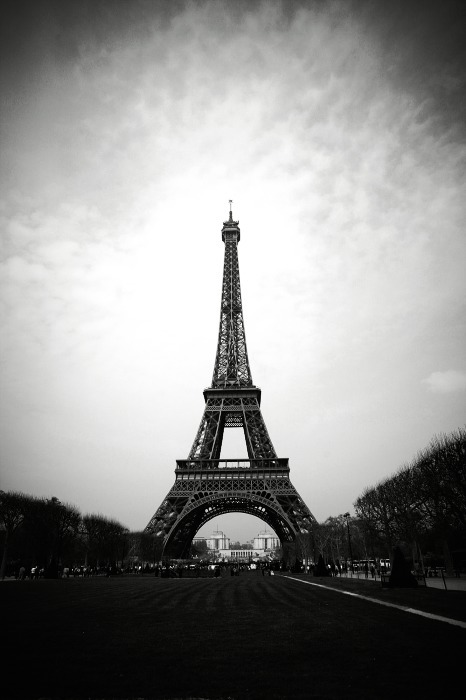
\includegraphics[width=5cm]{./images/tower.jpg}}}
    \qquad
    \subfloat[\centering Обработанное изображение]{{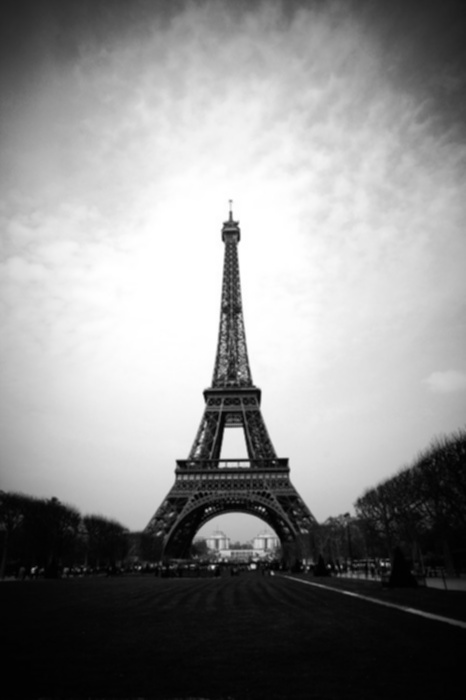
\includegraphics[width=5cm]{./images/tower1.jpg}}}
\end{figure}

\begin{figure}[H]
    \centering
    \subfloat[\centering Оригинальное изображение]{{
\includegraphics[width=5cm]{./images/unn_logo.png}}}
    \qquad
    \subfloat[\centering Обработанное изображение]{{
\includegraphics[width=5cm]{./images/unn_logo1.png}}}
\end{figure}
 


\newpage

\section*{Заключение}
\addcontentsline{toc}{section}{Заключение}

В данной лабораторной работе мы реализовали последовательную и паралелльные версии алгоритма линейной фильтрации изображений с ядром Гаусса 3х3. Итоговый прирост производительности составил 2.7 раза.

Так же мы смогли наглядно увидеть результат работы алгоритма на примерах.

\newpage

\begin{thebibliography}{1}
\addcontentsline{toc}{section}{Список литературы}
\bibitem{OMP} Гергель В.П. Учебный курс «Введение в методы параллельного программирования», раздел «Параллельное программирование с использованием OpenMP». Нижний Новгород, ННГУ, 2007.
\bibitem{TBB} А.А. Сиднев, А.В. Сысоев, И.Б. Мееров. Учебный курс «Технологии разработки параллельных программ», раздел «Создание параллельной программы», «Библиотека Intel Threading Building Blocks~--- краткое описание». Нижний Новгород, ННГУ, 2007. 
\end{thebibliography}

\newpage

\section*{Приложение}
\addcontentsline{toc}{section}{Приложение}


Последовательная версия:

\begin{lstlisting}[breaklines=true]
// lin_filter_vertical_part.h
// Copyright 2021 Tronin Dmitry
#ifndef MODULES_TASK_1_TRONIN_D_LIN_FILTER_VERTICAL_PART_LIN_FILTER_VERTICAL_PART_H_
#define MODULES_TASK_1_TRONIN_D_LIN_FILTER_VERTICAL_PART_LIN_FILTER_VERTICAL_PART_H_

#include <cstdint>
#include <vector>

std::vector<double> CalculateGaussFilter(size_t size, double sigma);
std::vector<uint8_t> ApplyFilter(const std::vector<double> &filter,
                                 const std::vector<uint8_t> &image,
                                 size_t width,
                                 size_t height,
                                 size_t filter_size);

template<class T>
T Clamp(T value, T low, T high) {
    if (value < low) {
        return low;
    }
    if (value > high) {
        return high;
    }
    return value;
}

#endif  // MODULES_TASK_1_TRONIN_D_LIN_FILTER_VERTICAL_PART_LIN_FILTER_VERTICAL_PART_H_

\end{lstlisting}

\begin{lstlisting}[breaklines=true]
// lin_filter_vertical_part.cpp
// Copyright 2021 Tronin Dmitry
#include "../../modules/task_1/tronin_d_lin_filter_vertical_part/lin_filter_vertical_part.h"

#include <cmath>
#include <stdexcept>

static const double kPi = 3.141592653589793;

std::vector<double> CalculateGaussFilter(size_t size, double sigma) {
    if (size % 2 == 0) {
        throw std::invalid_argument("Size can't be even");
    }
    if (size <= 0) {
        throw std::invalid_argument("Size should be positive");
    }
    if (sigma <= 0) {
        throw std::invalid_argument("Sigma should be positive");
    }
    double sum = 0;

    std::vector<double> filter(size * size, 0);
    for (int row = -static_cast<int>(size) / 2; row <= static_cast<int>(size) / 2; ++row) {
        for (int col = -static_cast<int>(size) / 2; col <= static_cast<int>(size) / 2; ++col) {
            filter[(row + static_cast<int>(size) / 2) * size + col + static_cast<int>(size) / 2] =
                1. / (2 * kPi * sigma * sigma)
                    * exp(-static_cast<double>(row * row + col * col) / (2 * sigma * sigma));
            sum += filter[(row + static_cast<int>(size) / 2) * size + col
                + static_cast<int>(size) / 2];
        }
    }

    double a = 0;

    for (int row = -static_cast<int>(size) / 2; row <= static_cast<int>(size) / 2; ++row) {
        for (int col = -static_cast<int>(size) / 2; col <= static_cast<int>(size) / 2; ++col) {
            filter[(row + static_cast<int>(size) / 2) * size + col + static_cast<int>(size) / 2] /=
                sum;
            a += filter[(row + static_cast<int>(size) / 2) * size + col
                + static_cast<int>(size) / 2];
        }
    }
    return filter;
}

std::vector<uint8_t> ApplyFilter(const std::vector<double> &filter,
                                 const std::vector<uint8_t> &image,
                                 size_t width,
                                 size_t height,
                                 size_t filter_size) {
    if (image.size() != width * height) {
        throw std::invalid_argument("Incorrect image size");
    }
    if (filter.size() != filter_size * filter_size) {
        throw std::invalid_argument("Incorrect filter size");
    }
    if (width <= 0 || height <= 0 || filter_size <= 0) {
        throw std::invalid_argument("Arguments should be positive");
    }
    std::vector<uint8_t> result_image(image.size());
    for (size_t row = 0; row < height; ++row) {
        for (size_t col = 0; col < width; ++col) {
            double pixel_value = 0;
            for (int filter_row = -static_cast<int>(filter_size) / 2;
                 filter_row <= static_cast<int>(filter_size) / 2; ++filter_row) {
                for (int filter_col = -static_cast<int>(filter_size) / 2;
                     filter_col <= static_cast<int>(filter_size) / 2; ++filter_col) {
                    auto image_row = static_cast<size_t>(Clamp(static_cast<int>(row) + filter_row,
                                                               0,
                                                               static_cast<int>(height) - 1));
                    auto image_col = static_cast<size_t>(Clamp(static_cast<int>(col) + filter_col,
                                                               0,
                                                               static_cast<int>(width) - 1));
                    double test = image[image_row * width + image_col]
                        * filter[(filter_row + static_cast<int>(filter_size) / 2) * filter_size
                            + filter_col + static_cast<int>(filter_size) / 2];
                    pixel_value += test;
                }
            }
            result_image[row * width + col] =
                static_cast<uint8_t>(Clamp(pixel_value, 0., 255.));
        }
    }
    return result_image;
}

\end{lstlisting}

Реализация с использование OpenMP:

\begin{lstlisting}[breaklines=true]
//lin_filter_vertical_part.h
// Copyright 2021 Tronin Dmitry
#ifndef MODULES_TASK_2_TRONIN_D_LIN_FILTER_VERTICAL_PART_LIN_FILTER_VERTICAL_PART_H_
#define MODULES_TASK_2_TRONIN_D_LIN_FILTER_VERTICAL_PART_LIN_FILTER_VERTICAL_PART_H_

#include <cstdint>
#include <vector>

std::vector<double> CalculateGaussFilterP(size_t size, double sigma);
std::vector<uint8_t> ApplyFilterParallel(const std::vector<double> &filter,
                                 const std::vector<uint8_t> &image,
                                 size_t width,
                                 size_t height,
                                 size_t filter_size);

template<class T>
inline T ClampP(T value, T low, T high) {
    if (value < low) {
        return low;
    }
    if (value > high) {
        return high;
    }
    return value;
}

#endif  // MODULES_TASK_2_TRONIN_D_LIN_FILTER_VERTICAL_PART_LIN_FILTER_VERTICAL_PART_H_
\end{lstlisting}

\begin{lstlisting}[breaklines=true]
//lin_filter_vertical_part.cpp
// Copyright 2021 Tronin Dmitry
#include "../../modules/task_2/tronin_d_lin_filter_vertical_part/lin_filter_vertical_part.h"
#include <omp.h>
#include <cmath>
#include <stdexcept>
#include <iostream>

static const double kPi = 3.141592653589793;

std::vector<double> CalculateGaussFilterP(size_t size, double sigma) {
    if (size % 2 == 0) {
        throw std::invalid_argument("Size can't be even");
    }
    if (size <= 0) {
        throw std::invalid_argument("Size should be positive");
    }
    if (sigma <= 0) {
        throw std::invalid_argument("Sigma should be positive");
    }
    double sum = 0;

    std::vector<double> filter(size * size, 0);
    for (int row = -static_cast<int>(size) / 2; row <= static_cast<int>(size) / 2; ++row) {
        for (int col = -static_cast<int>(size) / 2; col <= static_cast<int>(size) / 2; ++col) {
            filter[(row + static_cast<int>(size) / 2) * size + col + static_cast<int>(size) / 2] =
                1. / (2 * kPi * sigma * sigma)
                    * exp(-static_cast<double>(row * row + col * col) / (2 * sigma * sigma));
            sum += filter[(row + static_cast<int>(size) / 2) * size + col
                + static_cast<int>(size) / 2];
        }
    }

    double a = 0;

    for (int row = -static_cast<int>(size) / 2; row <= static_cast<int>(size) / 2; ++row) {
        for (int col = -static_cast<int>(size) / 2; col <= static_cast<int>(size) / 2; ++col) {
            filter[(row + static_cast<int>(size) / 2) * size + col + static_cast<int>(size) / 2] /=
                sum;
            a += filter[(row + static_cast<int>(size) / 2) * size + col
                + static_cast<int>(size) / 2];
        }
    }
    return filter;
}

std::vector<uint8_t> ApplyFilterParallel(const std::vector<double> &filter,
                                         const std::vector<uint8_t> &image,
                                         size_t width,
                                         size_t height,
                                         size_t filter_size) {
    if (image.size() != width * height) {
        throw std::invalid_argument("Incorrect image size");
    }
    if (filter.size() != filter_size * filter_size) {
        throw std::invalid_argument("Incorrect filter size");
    }
    if (width <= 0 || height <= 0 || filter_size <= 0) {
        throw std::invalid_argument("Arguments should be positive");
    }
    std::vector<uint8_t> result_image(image.size(), 1);

    double pixel_value, test;
    int image_row, image_col;

#pragma omp parallel default(none) shared(image, width, height, filter_size, filter, result_image, std::cout)
    {
#pragma omp for private(pixel_value, test, image_row, image_col)
        for (int col = 0; col < static_cast<int>(width); ++col) {
            for (int row = 0; row < static_cast<int>(height); ++row) {
                pixel_value = 0;
                for (int filter_row = -static_cast<int>(filter_size) / 2;
                     filter_row <= static_cast<int>(filter_size) / 2; ++filter_row) {
                    for (int filter_col = -static_cast<int>(filter_size) / 2;
                         filter_col <= static_cast<int>(filter_size) / 2; ++filter_col) {
                        image_row =
                            static_cast<size_t>(ClampP(static_cast<int>(row) + filter_row,
                                                       0,
                                                       static_cast<int>(height) - 1));
                        image_col =
                            static_cast<size_t>(ClampP(static_cast<int>(col) + filter_col,
                                                       0,
                                                       static_cast<int>(width) - 1));
                        test = image[image_row * width + image_col]
                            * filter[
                                (filter_row + static_cast<int>(filter_size) / 2) * filter_size
                                    + filter_col + static_cast<int>(filter_size) / 2];
                        pixel_value += test;
                    }
                }
                result_image[row * width + col] =
                    static_cast<uint8_t>(ClampP(pixel_value, 0., 255.));
            }
        }
    }

    return result_image;
}

\end{lstlisting}

Реализация с помощью TBB:

\begin{lstlisting}[breaklines=true]
//lin_filter_vertical_part.h
// Copyright 2021 Tronin Dmitry
#ifndef MODULES_TASK_3_TRONIN_D_LIN_FILTER_VERTICAL_PART_LIN_FILTER_VERTICAL_PART_H_
#define MODULES_TASK_3_TRONIN_D_LIN_FILTER_VERTICAL_PART_LIN_FILTER_VERTICAL_PART_H_

#include <cstdint>
#include <vector>
#include <tbb/tbb.h>
#include "tbb/parallel_for.h"
#include "tbb/blocked_range.h"

std::vector<double> CalculateGaussFilterTBB(size_t size, double sigma);
std::vector<uint8_t> ApplyFilterTBB(const std::vector<double> &filter,
                                    const std::vector<uint8_t> &image,
                                    size_t width,
                                    size_t height,
                                    size_t filter_size, size_t number_of_threads);

template<class T>
inline T ClampTBB(T value, T low, T high) {
    if (value < low) {
        return low;
    }
    if (value > high) {
        return high;
    }
    return value;
}

#endif  // MODULES_TASK_2_TRONIN_D_LIN_FILTER_VERTICAL_PART_LIN_FILTER_VERTICAL_PART_H_
\end{lstlisting}

\begin{lstlisting}[breaklines=true]
//lin_filter_vertical_part.cpp
// Copyright 2021 Tronin Dmitry
#include "../../modules/task_3/tronin_d_lin_filter_vertical_part/lin_filter_vertical_part.h"
#include <cmath>
#include <stdexcept>
#include <iostream>
#include <atomic>

static const double kPi = 3.141592653589793;

std::vector<double> CalculateGaussFilterTBB(size_t size, double sigma) {
    if (size % 2 == 0) {
        throw std::invalid_argument("Size can't be even");
    }
    if (size <= 0) {
        throw std::invalid_argument("Size should be positive");
    }
    if (sigma <= 0) {
        throw std::invalid_argument("Sigma should be positive");
    }
    double sum = 0;

    std::vector<double> filter(size * size, 0);
    for (int row = -static_cast<int>(size) / 2; row <= static_cast<int>(size) / 2; ++row) {
        for (int col = -static_cast<int>(size) / 2; col <= static_cast<int>(size) / 2; ++col) {
            filter[(row + static_cast<int>(size) / 2) * size + col + static_cast<int>(size) / 2] =
                1. / (2 * kPi * sigma * sigma)
                    * exp(-static_cast<double>(row * row + col * col) / (2 * sigma * sigma));
            sum += filter[(row + static_cast<int>(size) / 2) * size + col
                + static_cast<int>(size) / 2];
        }
    }

    double a = 0;

    for (int row = -static_cast<int>(size) / 2; row <= static_cast<int>(size) / 2; ++row) {
        for (int col = -static_cast<int>(size) / 2; col <= static_cast<int>(size) / 2; ++col) {
            filter[(row + static_cast<int>(size) / 2) * size + col + static_cast<int>(size) / 2] /=
                sum;
            a += filter[(row + static_cast<int>(size) / 2) * size + col
                + static_cast<int>(size) / 2];
        }
    }
    return filter;
}

std::vector<uint8_t> ApplyFilterTBB(const std::vector<double> &filter,
                                    const std::vector<uint8_t> &image,
                                    size_t width,
                                    size_t height,
                                    size_t filter_size, size_t number_of_threads) {
    if (image.size() != width * height) {
        throw std::invalid_argument("Incorrect image size");
    }
    if (filter.size() != filter_size * filter_size) {
        throw std::invalid_argument("Incorrect filter size");
    }
    if (width <= 0 || height <= 0 || filter_size <= 0) {
        throw std::invalid_argument("Arguments should be positive");
    }
    std::vector<uint8_t> result_image(image.size(), 1);

    tbb::task_scheduler_init init(static_cast<int>(number_of_threads));

    tbb::parallel_for(tbb::blocked_range<int>(0,
                                              static_cast<int>(width),
                                              width / number_of_threads),
                      [height, width, &image, &result_image, filter_size, &filter](tbb::blocked_range<
                          int> r) {

                        for (int col = r.begin(); col != r.end(); ++col) {
                            for (int row = 0; row < static_cast<int>(height); ++row) {

                                double pixel_value = 0;
                                for (int filter_row = -static_cast<int>(filter_size) / 2;
                                     filter_row <= static_cast<int>(filter_size) / 2;
                                     ++filter_row) {
                                    for (int filter_col = -static_cast<int>(filter_size) / 2;
                                         filter_col <= static_cast<int>(filter_size) / 2;
                                         ++filter_col) {
                                        size_t image_row =
                                            static_cast<size_t>(ClampTBB(
                                                static_cast<int>(row) + filter_row,
                                                0,
                                                static_cast<int>(height) - 1));
                                        size_t image_col =
                                            static_cast<size_t>(ClampTBB(
                                                static_cast<int>(col) + filter_col,
                                                0,
                                                static_cast<int>(width) - 1));
                                        double test = image[image_row * width + image_col]
                                            * filter[
                                                (filter_row + static_cast<int>(filter_size) / 2)
                                                    * filter_size
                                                    + filter_col
                                                    + static_cast<int>(filter_size) / 2];
                                        pixel_value += test;
                                    }
                                }
                                result_image[row * width + col] =
                                    static_cast<uint8_t>(ClampTBB(pixel_value, 0., 255.));
                            }
                        }
                      });

    return result_image;
}
\end{lstlisting}

Реализация с помощью \verb|std::thread|:

\begin{lstlisting}[breaklines=true]
//lin_filter_vertical_part.h
// Copyright 2021 Tronin Dmitry
#ifndef MODULES_TASK_4_TRONIN_D_LIN_FILTER_VERTICAL_PART_LIN_FILTER_VERTICAL_PART_H_
#define MODULES_TASK_4_TRONIN_D_LIN_FILTER_VERTICAL_PART_LIN_FILTER_VERTICAL_PART_H_

#include <cstdint>
#include <vector>

std::vector<double> CalculateGaussFilterSTD(size_t size, double sigma);
std::vector<uint8_t> ApplyFilterSTD(const std::vector<double> &filter,
                                    const std::vector<uint8_t> &image,
                                    size_t width,
                                    size_t height,
                                    size_t filter_size, size_t number_of_threads);

template<class T>
inline T ClampSTD(T value, T low, T high) {
    if (value < low) {
        return low;
    }
    if (value > high) {
        return high;
    }
    return value;
}

#endif  // MODULES_TASK_4_TRONIN_D_LIN_FILTER_VERTICAL_PART_LIN_FILTER_VERTICAL_PART_H_
\end{lstlisting}

\begin{lstlisting}[breaklines=true]
//lin_filter_vertical_part.cpp
// Copyright 2021 Tronin Dmitry
#include "../../modules/task_4/tronin_d_lin_filter_vertical_part/lin_filter_vertical_part.h"
#include <cmath>
#include <stdexcept>
#include <iostream>
#include <thread>

static const double kPi = 3.141592653589793;

std::vector<double> CalculateGaussFilterSTD(size_t size, double sigma) {
    if (size % 2 == 0) {
        throw std::invalid_argument("Size can't be even");
    }
    if (size <= 0) {
        throw std::invalid_argument("Size should be positive");
    }
    if (sigma <= 0) {
        throw std::invalid_argument("Sigma should be positive");
    }
    double sum = 0;

    std::vector<double> filter(size * size, 0);
    for (int row = -static_cast<int>(size) / 2; row <= static_cast<int>(size) / 2; ++row) {
        for (int col = -static_cast<int>(size) / 2; col <= static_cast<int>(size) / 2; ++col) {
            filter[(row + static_cast<int>(size) / 2) * size + col + static_cast<int>(size) / 2] =
                1. / (2 * kPi * sigma * sigma)
                    * exp(-static_cast<double>(row * row + col * col) / (2 * sigma * sigma));
            sum += filter[(row + static_cast<int>(size) / 2) * size + col
                + static_cast<int>(size) / 2];
        }
    }

    double a = 0;

    for (int row = -static_cast<int>(size) / 2; row <= static_cast<int>(size) / 2; ++row) {
        for (int col = -static_cast<int>(size) / 2; col <= static_cast<int>(size) / 2; ++col) {
            filter[(row + static_cast<int>(size) / 2) * size + col + static_cast<int>(size) / 2] /=
                sum;
            a += filter[(row + static_cast<int>(size) / 2) * size + col
                + static_cast<int>(size) / 2];
        }
    }
    return filter;
}

std::vector<uint8_t> ApplyFilterSTD(const std::vector<double> &filter,
                                    const std::vector<uint8_t> &image,
                                    size_t width,
                                    size_t height,
                                    size_t filter_size, size_t number_of_threads) {
    if (image.size() != width * height) {
        throw std::invalid_argument("Incorrect image size");
    }
    if (filter.size() != filter_size * filter_size) {
        throw std::invalid_argument("Incorrect filter size");
    }
    if (width <= 0 || height <= 0 || filter_size <= 0) {
        throw std::invalid_argument("Arguments should be positive");
    }
    std::vector<uint8_t> result_image(image.size(), 1);

    std::vector<std::thread> threads;

    for (size_t i = 0; i < number_of_threads; ++i) {
        threads.emplace_back([width, height, number_of_threads, &image, &result_image, filter_size, &filter, i]() {
          for (int col = static_cast<int>(width) / number_of_threads * i;
               col < static_cast<int>(width) / number_of_threads * (i + 1)
                   + (i == number_of_threads ? width % number_of_threads : 0); ++col) {
              for (int row = 0; row < static_cast<int>(height); ++row) {
                  double pixel_value = 0;
                  for (int filter_row = -static_cast<int>(filter_size) / 2;
                       filter_row <= static_cast<int>(filter_size) / 2;
                       ++filter_row) {
                      for (int filter_col =
                          -static_cast<int>(filter_size) / 2;
                           filter_col <= static_cast<int>(filter_size) / 2;
                           ++filter_col) {
                          size_t image_row =
                              static_cast<size_t>(ClampSTD(
                                  static_cast<int>(row) + filter_row,
                                  0,
                                  static_cast<int>(height) - 1));
                          size_t image_col =
                              static_cast<size_t>(ClampSTD(
                                  static_cast<int>(col) + filter_col,
                                  0,
                                  static_cast<int>(width) - 1));
                          double test = image[image_row * width + image_col]
                              * filter[
                                  (filter_row
                                      + static_cast<int>(filter_size) / 2)
                                      * filter_size
                                      + filter_col
                                      + static_cast<int>(filter_size) / 2];
                          pixel_value += test;
                      }
                  }
                  result_image[row * width + col] =
                      static_cast<uint8_t>(ClampSTD(pixel_value, 0., 255.));
              }
          }
        });
    }

    for (auto &thread : threads) {
        thread.join();
    }

    return result_image;
}
\end{lstlisting}

Приложение дял визуализации (для последовательной версии, для других реализаций приложение выглядит аналогично):

\begin{lstlisting}
#include <opencv2/core.hpp>
#include <opencv2/imgcodecs.hpp>
#include <opencv2/imgproc.hpp>
#include <vector>
#include <iostream>

#include "../task_1/tronin_d_lin_filter_vertical_part/lin_filter_vertical_part.h"

using namespace cv;

int main(int argc, char *argv[]) {
    if (argc < 4) {
        std::cerr << "Usage: " << argv[0] << " input_file output_file sigma" << std::endl;
        return 1;
    }

    Mat img = imread(argv[1], IMREAD_GRAYSCALE);
    if (img.empty()) {
        std::cout << "Could not read the image: " << argv[1] << std::endl;
        return 1;
    }


    std::vector<uchar> array(img.datastart, img.dataend);

    auto app =
        ApplyFilter(CalculateGaussFilter(3, std::stod(argv[3])), array, img.cols, img.rows, 3);

    Mat new_img(img.rows, img.cols, CV_8U, app.data());

    imwrite(argv[2], new_img);

    std::cout << "Image saved: " << argv[2] << std::endl;

    return 0;
}
\end{lstlisting}

Приложение для вычислительных экспериментов:

\begin{lstlisting}[breaklines=true]
#include <benchmark/benchmark.h>
#include "../task_4/tronin_d_lin_filter_vertical_part/lin_filter_vertical_part.h"
#include "../task_3/tronin_d_lin_filter_vertical_part/lin_filter_vertical_part.h"
#include "../task_2/tronin_d_lin_filter_vertical_part/lin_filter_vertical_part.h"
#include "../task_1/tronin_d_lin_filter_vertical_part/lin_filter_vertical_part.h"
#include <opencv2/core.hpp>
#include <opencv2/imgcodecs.hpp>
#include <opencv2/imgproc.hpp>
#include <vector>
#include <omp.h>

#include <iostream>

using namespace cv;

const static std::string file{"tree.jpg"};

void ImageProcessParallelOMP(benchmark::State &state) {
    for (auto _ : state) {

        Mat img = imread(file, IMREAD_GRAYSCALE);
        std::vector<uint8_t> image(img.datastart, img.dataend);

        omp_set_num_threads(state.range());

        double start = omp_get_wtime();

        auto res = ApplyFilterParallel(CalculateGaussFilterP(3, 1.0),
                                        image,
                                        img.cols,
                                        img.rows,
                                        3);

        double stop = omp_get_wtime();

        state.SetIterationTime(stop - start);
    }
}


void ImageProcessParallelTBB(benchmark::State &state) {
    for (auto _ : state) {
        Mat img = imread(file, IMREAD_GRAYSCALE);
        std::vector<uint8_t> image(img.datastart, img.dataend);

        tbb::tick_count start = tbb::tick_count::now();

        auto res = ApplyFilterTBB(CalculateGaussFilterTBB(3, 1.0),
                                        image,
                                        img.cols,
                                        img.rows,
                                        3,
                                        state.range());

        tbb::tick_count stop = tbb::tick_count::now();


        state.SetIterationTime((stop - start).seconds());
    }
}


void ImageProcessParallelSTD(benchmark::State &state) {
    for (auto _ : state) {
        Mat img = imread(file, IMREAD_GRAYSCALE);
        std::vector<uint8_t> image(img.datastart, img.dataend);

        auto start = std::chrono::high_resolution_clock::now();

        auto res = ApplyFilterSTD(CalculateGaussFilterSTD(3, 1.0),
                                    image,
                                    img.cols,
                                    img.rows,
                                    3,
                                    state.range());

        auto stop = std::chrono::high_resolution_clock::now();


        state.SetIterationTime( std::chrono::duration<double>(stop - start).count());
    }


}

BENCHMARK(ImageProcessParallelOMP)->UseManualTime()->Unit(benchmark::kSecond)->DenseRange(1, 8, 1)->Iterations(10);
BENCHMARK(ImageProcessParallelTBB)->UseManualTime()->Unit(benchmark::kSecond)->DenseRange(1, 8, 1)->Iterations(10);
BENCHMARK(ImageProcessParallelSTD)->UseManualTime()->Unit(benchmark::kSecond)->DenseRange(1, 8, 1)->Iterations(10);

void ImageProcessSeq(benchmark::State &state) {
    for (auto _ : state) {
        Mat img = imread(file, IMREAD_GRAYSCALE);
        std::vector<uint8_t> image(img.datastart, img.dataend);

        double start = omp_get_wtime();

        auto res = ApplyFilter(CalculateGaussFilter(3, 1.0), image, img.cols, img.rows, 3);

        double stop = omp_get_wtime();

        state.SetIterationTime(stop - start);
    }

}

BENCHMARK(ImageProcessSeq)->UseManualTime()->Unit(benchmark::kSecond);
BENCHMARK_MAIN();

\end{lstlisting}
\end{document}